\documentclass[12pt]{article}
\usepackage[utf8]{inputenc}
\usepackage{amsmath}
\usepackage{graphicx}
\usepackage{array}
\usepackage{geometry}
\geometry{margin=2.5cm}
\usepackage{titlesec}
\usepackage{float}
\titleformat{\section}{\centering\bfseries\uppercase}{\thesection}{1em}{}

\begin{document}

\section*{ DISEÑO A FLEXIÓN DE VIGA 30X50 }

\begin{minipage}[t]{0.48\textwidth}
\begin{tabular}{|l|c|}
\hline
Base (b) &  m \\
Altura (h) &  m \\
Recubrimiento (r) &  m \\
Estribo (\ensuremath{\phi_e}) &  m \\
Varilla principal (\ensuremath{\phi_s}) &  m \\
f'c &  MPa \\
fy &  MPa \\
\hline
\end{tabular}
\end{minipage}
\hfill
\begin{minipage}[t]{0.48\textwidth}

\begin{figure}[H]
\centering
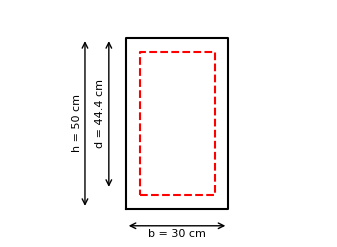
\includegraphics[height=5cm]{c:/Users/PC/Desktop/LOCAL REPOSITORIE/VIGA_FINAL/src/vigapp/ui/../../pdf_engine/figures/section.png}
\end{figure}

\end{minipage}

\vspace{0.5cm}

\section*{Peralte: d (ART.PERALTE)}

\[

\]

Valor calculado: \( d = \,\text{m} \)



\vspace{0.5cm}

\section*{Coeficiente B1 (ART.B1)}

\[

\]

Valor calculado: \( \beta_1 =  \)



\vspace{0.5cm}

\section*{Pbal (ART.PBAL)}

\[

\]

Valor calculado: \( P_{bal} =  \)



\vspace{0.5cm}

\section*{\ensuremath{\rho_{bal}} (ART.RHOBAL)}

\[

\]

Valor calculado: \( \rho_{bal} =  \)



\vspace{0.5cm}

\section*{Pmax (ART.PMAX)}

\[

\]

Valor calculado: \( P_{max} =  \)



\vspace{0.5cm}

\section*{As m\'in (ART.ASMIN)}

\[

\]

Valor calculado: \( A_{s}^{\text{min}} =  \)



\vspace{0.5cm}

\section*{As m\'ax (ART.ASMAX)}

\[

\]

Valor calculado: \( A_{s}^{\text{max}} =  \)



\end{document}